\chapter{Introduzione}

% Data Analytics
% TODO: descrizione

\begin{figure}[ht]
  \centering
  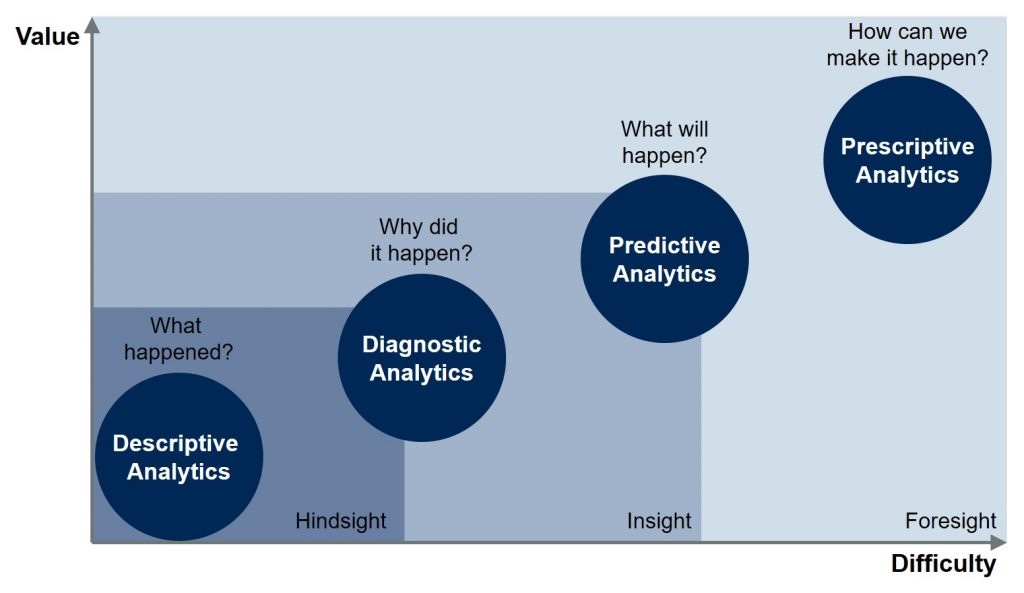
\includegraphics[width=0.8\textwidth]{images/GartnerFourAnalyticTypesV5-1024x593.jpg}
  \caption{Diversi tipi di analisi per valore e difficoltà \cite{web:GartnerFourAnalyticTypesV5}.}
\end{figure}

\pagebreak

\section{Definizioni}

Un'\textbf{istanza} (instance, item, record) é un esempio descritto da un insieme finito di attributi.
Il numero di attributi può variare per alcune istanze.

Un \textbf{attributo} (attribute, field, variable) é una misura di un aspetto
di un'istanza.

Tipi di attributi:
\begin{itemize}
  \item \textbf{Quantità nominali}: i valori sono \textbf{simboli} distinti. Non hanno relazioni come ordinamento o distanza.\\(e.g. attributo: ``outlook'', valori: ``sunny”, ``cloudy'', and ``rainy'').
  \item \textbf{Quantità ordinali}: i valori hanno una relazione d'ordine, ma non di distanza.\\(e.g. attributo: ``temperature'', valori: ``hot'' $>$ ``mild'' $>$ ``cold'').
  \item \textbf{Quantità d'intervallo}: 
  \item \textbf{Quantità di rapporto}: 
\end{itemize}

Una \textbf{classe} (class, label) rappresenta un gruppo di istanze che condividono delle caratteristiche comuni.

\subsection*{Propositionalization}
% TODO: descrizione

\begin{figure}[ht]
  \centering
  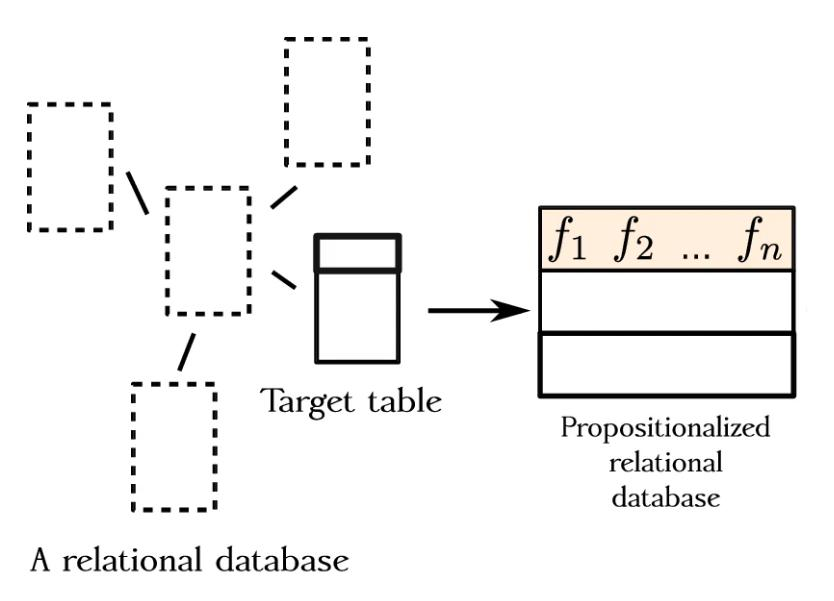
\includegraphics[width=0.5\textwidth]{images/Propositionalization.jpeg}
  \caption{Processo di propositionalization \cite{lavravc2020propositionalization}}
\end{figure}

\pagebreak

\section{Pre-Processing}
I dati nel mondo reale sono \textbf{incompleti}, \textbf{rumorosi} e \textbf{inconsistenti}.
Per ottenere dell'analisi di qualità é necessario effettuare prima delle 
operazioni sui dati.

\begin{itemize}
  \item \textbf{Data Cleaning}: sostituire valori mancanti, smussare dati rumorosi, identificare o rimuovere outliers e risolvere inconsistenze.
  \item \textbf{Data Integration}: integrazione di diversi dati.
  \item \textbf{Data Transformation}: normalizzare o aggregare i dati
  \item \textbf{Data Reduction}: feature selection, feature extraction
\end{itemize}

\section{Data Cleaning}

\subsection*{Dati Mancanti}
Alcuni dati possono non essere stati calcolati o possono non essere disponibili per malfunzionamenti o per errori umani.

L'assenza di questi dati \textbf{complica l'analisi} poiché non tutti i metodi di analisi non gestiscono questo problema, 
inoltre comporta una \textbf{perdita di efficacia} nell'estrarre dei pattern.

Categorie di valori mancanti:
\begin{itemize}
  % TODO: descrizione
  \item \textbf{Missing Completely At Random (MCAR)}:
  \item \textbf{Missing At Random (MAR)}:
  \item \textbf{Not Missing At Random (NMAR)}:
\end{itemize}

Gestione dei valori mancanti:
\begin{itemize}
  \item \textbf{Ignorare} le istanze o gli attributi con valori mancanti. 
  Praticabile solo se ci sono pochi esempi mancanti poiché introdurrebbe un bias.
  \item \textbf{Convertire} i valori mancanti in un nuovo valore (``missing'', ``?'', ``NA'').
  \item \textbf{Imputare} i valori mancanti basandosi sul resto del dataset. 
\end{itemize}

\subsubsection*{Metodi di Imputazione}
\begin{itemize}
  \item \textbf{Most Common (MC) Value}\\
  \underline{Assunzione}: ogni attributo ha una distribuzione normale.
  \begin{itemize}
    \item Valori \textbf{continui}: rimpiazza con la media dell'attributo nel dataset
    \item Valori \textbf{discreti}: rimpiazza con il valore più frequente dell'attributo nel dataset
  \end{itemize}

  \item \textbf{Concept Most Common (CMC) Value}\\
  \underline{Assunzione}: ogni attributo ha una distribuzione normale per tutte le istanze che appartengono alla stessa classe.

  I valori mancanti vengono rimpiazzati con il valore medio/più frequente delle istanze della stessa \textbf{classe}. 

  \item \textbf{K-Nearest Neighbors}\\
  Le istanze vengono disposte in uno spazio metrico e i valori mancanti vengono imputati considerando le k
istanze più vicine.
\end{itemize}

\subsection*{Dati Rumorosi}
Alcuni dati possono avere errori dovuti a \textbf{strumenti difettosi}, \textbf{errori umani} o \textbf{di calcolo}, 
errori durante la \textbf{trasmissione} dei dati o \textbf{limitazioni tecnologiche}. 

Questi errori introducono del ``rumore'' all'interno dei dati che può essere rimosso usando tecniche di \textbf{data smoothing}.
Queste tecniche riducono il rumore e rendono i pattern più identificabili, tuttavia si riduce la quantità di dati da analizzare e inoltre gli outliers possono alterare l'analisi. 

\subsubsection*{Binning}
I dati vengono \textbf{ordinati} e \textbf{partizionati} in bin. Quindi ogni bin si può smussare con media, mediana dei valori all'interno o utilizzando gli estremi. 

\begin{itemize}
  \item \textbf{Equal-width} (distance) partitioning: viene diviso il range in N intervalli di uguale dimensione. 
  \item \textbf{Equal-depth} (frequency) partitioning: viene diviso il range in N intervalli, ognuno dei quali contiene approssimatamene lo stesso numero di esempi.
\end{itemize}

% TODO: aggiungere degli esempi

\subsection*{Dati Sbilanciati}
Esistono molti problemi di classificazione in cui una classe ha una distribuzione fortemente sbilanciata, ovvero che il numero di 
osservazioni per una classe è molto inferiore a un'altra  (e.g. fraud detection, disease diagnosis, natural disaster, etc.). 
Quindi risulta difficile ottenere buoni valori di accuracy su entrambe le classi.

Un possibile approccio è quello di bilanciare i dati del train set.
\begin{itemize}
  \item \textbf{Oversampling}: aggiungere istanze alla \textbf{classe minoritaria} tramite campionamento con rimpiazzo (i.e. duplicare alcuni valori) fino a ottenere lo stesso numero di istanze per classe.
  Bilancia le classi, ma non fornisce nuove informazioni al modello.
  \item \textbf{Undersampling}: rimuovere randomicamente istanze dalla \textbf{classe maggioritaria} fino a ottenere lo stesso numero di istanze per classe.
\end{itemize}

\begin{figure}[ht]
  \centering
  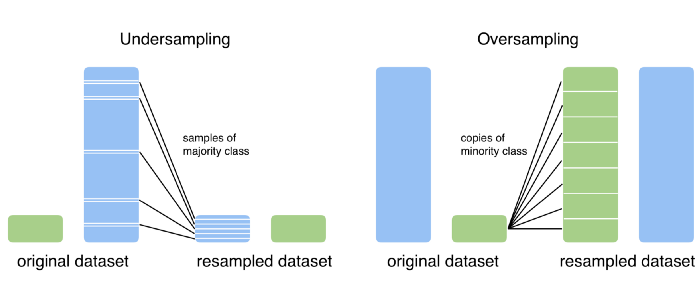
\includegraphics[width=\textwidth]{images/resampling.png}
  \caption{Rappresentazione del funzionamento del random resampling.}
\end{figure}

\subsubsection*{Synthetic Minority Oversampling Technique (SMOTE)}
SMOTE è una tecnica di oversampling che genera esempi sintetici della classe minoritaria a partire dai dati esistenti.
Dato un esempio della classe minoritaria vengono selezionati i k esempi più vicini, viene scelto uno a caso tra questi e
viene generato un numero esempio tra questi due.
% TODO: spiegare meglio
% TODO: immagine

\subsubsection*{Tomek Links}
Tomek Links è una tecnica di undersampling che rimuove gli esempi della classe maggioritaria che appartengono a un Tomek Link.
Un \textbf{Tomek Link} é una coppia d'istanze $(E_i, E_j)$ di classi diverse per cui non esiste nessun'altra istanza che sia più vicina 
a uno dei due.

La collezione di Tomek Links nel dataset definisce le frontiere delle classi.
\begin{figure}[ht]
  \centering
  
\includegraphics[width=0.9\textwidth]{images/tomeklinks.png}
  \caption{Esempio di undersampling tramite Tomek Links \cite{web:TomekLinks}.}
\end{figure}

% \section{Data Reduction}
% NEXT
